\documentclass[10pt]{book}
\usepackage{makeidx}
\makeindex
%\usepackage{showidx}
% mark overful hboxes
%\overfullrule=1mm
\usepackage{kpfonts}

%\usepackage[nott]{kpfonts}
%\SetMathAlphabet{\mathtt}{normal}{OT1}{\ttdefault}{m}{n}
%\SetMathAlphabet{\mathtt}{bold}{OT1}{\ttdefault}{m}{n}

%\usepackage[math]{iwona}
%\SetMathAlphabet{\mathtt}{iwona}{OT1}{\ttdefault}{m}{n}
%\usepackage[T1]{fontenc}

\usepackage{amsopn}
\usepackage{amsmath}
\usepackage{amsthm}
\usepackage{url}
\usepackage{graphicx}
\usepackage{datetime}
\usepackage{amsfonts}
\usepackage{graphicx}
\usepackage{threeparttable}
\usepackage{wasysym}
\usepackage{emptypage}

%% This code allows dynamic scaling of images to fit the page
%% Usage: \includegraphics[width=\ScaleIfNeeded]{figs/figure}
\makeatletter
\def\ScaleIfNeeded{%
\ifdim\Gin@nat@width>.97\linewidth
.97\linewidth
\else
\Gin@nat@width
\fi
}
\makeatother

\makeatletter
\def\HalfScaleIfNeeded{%
\ifdim\Gin@nat@width>.46\linewidth
.46\linewidth
\else
\Gin@nat@width
\fi
}
\makeatother

\makeatletter
\def\HeightScaleIfNeeded{%
\ifdim\Gin@nat@height>.8\textheight
.8\textheight
\else
\Gin@nat@height
\fi
}
\makeatother


\makeatletter
\def\QuarterHeightScaleIfNeeded{%
\ifdim\Gin@nat@height>.22\textheight
.22\textheight
\else
\Gin@nat@height
\fi
}
\makeatother

\makeatletter
\def\FifthHeightScaleIfNeeded{%
\ifdim\Gin@nat@height>.168\textheight
.168\textheight
\else
\Gin@nat@height
\fi
}
\makeatother



%\usepackage[mathlines]{lineno}
%\linenumbers
%\DeclareGraphicsExtensions{.pdf,.eps}

% Leave this here - it gets substituted with language specific stuff
%HEADCOMMAND

\allowdisplaybreaks[1]  % for ams math align environments

\hyphenation{Array-Stack}
\hyphenation{Fast-Array-Stack}
\hyphenation{Array-Queue}
\hyphenation{Array-Deque}
\hyphenation{Dual-Array-Deque}
\hyphenation{Root-ish-Array-Stack}
\hyphenation{Skip-list-Set}
\hyphenation{Skip-list-List}
\hyphenation{Hash-Table}
\hyphenation{Chained-Hash-Table}
\hyphenation{Linear-Hash-Table}
\hyphenation{Red-Black-Tree}
\hyphenation{Binary-Tree}
\hyphenation{Binary-Search-Tree}
\hyphenation{Scape-goat-Tree}
\hyphenation{Binary-Heap}
\hyphenation{Meld-able-Heap}
\hyphenation{Java-Script}

\usepackage{everysel}
\EverySelectfont{%
%\fontdimen2\font=0.4em% interword space
%\fontdimen3\font=0.2em% interword stretch
%\fontdimen4\font=0.1em% interword shrink
%\fontdimen7\font=0.1em% extra space
\hyphenchar\font=`\-% to allow hyphenation
}

\usepackage[sf,small,raggedright]{titlesec} % formatting titles
\titlespacing*{\section}{0pt}{24pt}{14pt}
\titlespacing*{\subsection}{0pt}{14pt}{14pt}
\usepackage{relsize,fancyvrb}  % formatting pseudocode
\usepackage{ods} % Personalization and commands

\htmlonly{
\newcommand{\ScaleIfNeeded}{\textwidth}
\newcommand{\HalfScaleIfNeeded}{\textwidth}
}

%\newcommand{\comment}[1]{}
\newcommand{\chaplabel}[1]{\label{chap:#1}}
\newcommand{\Chapref}[1]{Chapter~\ref{chap:#1}}
\newcommand{\chapref}[1]{Chapter~\ref{chap:#1}}
\newcommand{\seclabel}[1]{\label{sec:#1}}
\newcommand{\Secref}[1]{Section~\ref{sec:#1}}
\newcommand{\secref}[1]{Section~\ref{sec:#1}}
\newcommand{\sref}[1]{\textsection~\ref{sec:#1}}

\newcommand{\alglabel}[1]{\label{alg:#1}}
\newcommand{\Algref}[1]{Algorithm~\ref{alg:#1}}
\newcommand{\algref}[1]{Algorithm~\ref{alg:#1}}

\newcommand{\applabel}[1]{\label{app:#1}}
\newcommand{\Appref}[1]{Appendix~\ref{app:#1}}
\newcommand{\appref}[1]{Appendix~\ref{app:#1}}

\newcommand{\tablabel}[1]{\label{tab:#1}}
\newcommand{\Tabref}[1]{Table~\ref{tab:#1}}
\newcommand{\tabref}[1]{Table~\ref{tab:#1}}

\newcommand{\figlabel}[1]{\label{fig:#1}}
\newcommand{\Figref}[1]{Figure~\ref{fig:#1}}
\newcommand{\figref}[1]{Figure~\ref{fig:#1}}

\newcommand{\eqlabel}[1]{\label{eq:#1}}
\newcommand{\myeqref}[1]{(\ref{eq:#1})}
\newcommand{\Eqref}[1]{Equation~(\ref{eq:#1})}

\theoremstyle{plain}
\newtheorem{thm}{Theorem}[chapter]
\newcommand{\thmlabel}[1]{\label{thm:#1}}
\newcommand{\thmref}[1]{Theorem~\ref{thm:#1}}

\newtheorem{lem}{Lemma}[chapter]
\newcommand{\lemlabel}[1]{\label{lem:#1}}
\newcommand{\lemref}[1]{Lemma~\ref{lem:#1}}

\newtheorem{cor}{Corollary}[chapter]
\newcommand{\corlabel}[1]{\label{cor:#1}}
\newcommand{\corref}[1]{Corollary~\ref{cor:#1}}

\theoremstyle{definition}

\newtheorem{exc}{Exercise}[chapter]
\newcommand{\exclabel}[1]{\label{exc:#1}}
\newcommand{\excref}[1]{Exercise~\ref{exc:#1}}


\newtheorem{prp}{Property}[chapter]
\newcommand{\prplabel}[1]{\label{prp:#1}}
\newcommand{\prpref}[1]{Property~\ref{prp:#1}}

\newcommand{\etal}{\emph{et al.}}

\newcommand{\voronoi}{Vorono\u\i}
\newcommand{\ceil}[1]{{\lceil #1 \rceil}}
\newcommand{\Ceil}[1]{{\left\lceil #1 \right\rceil}}
\newcommand{\floor}[1]{{\lfloor #1 \rfloor}}
\newcommand{\Floor}[1]{{\left\lfloor #1 \right\rfloor}}
\newcommand{\R}{\mathbb{R}}
\newcommand{\N}{\mathbb{N}}
\newcommand{\Z}{\mathbb{Z}}
\newcommand{\Sp}{\mathbb{S}}
\newcommand{\E}{\mathrm{E}}
\DeclareMathOperator{\ddiv}{div}

% Colors for syntax highlighting
\usepackage[usenames,dvipsnames]{xcolor}
\definecolor{keyword}{named}{RoyalPurple}
\definecolor{var}{rgb}{0,0,0.5}   % Navy
\definecolor{comment}{named}{ForestGreen}
\definecolor{linkblue}{rgb}{.098,.098,.439} %Midnight blue
\definecolor{fm}{named}{ForestGreen}

\usepackage{tikz,gnuplot-lua-tikz}

\usepackage{hyperref}
\hypersetup{colorlinks=true, linkcolor=linkblue,  anchorcolor=linkblue,%
	citecolor=linkblue, filecolor=linkblue, menucolor=linkblue,%
	urlcolor=linkblue} 

% Title page content
\title{Open Data Structures}
\author{Pat Morin}
\date{%Development Edition: \today\ \currenttime
Edition 0.1E\cpponly{$\beta$}
\htmlonly{\\ 
\includegraphics[scale=0.90909,scale=0.5]{images/cc-by}}}
%Version 0.0 pre $\alpha$: \today}

\pagenumbering{roman}

% Draft mode only - mark overfull hboxes
% \overfullrule=5pt

\begin{document}

%%\AddToShipoutPicture*{\BackgroundPic}
%\begin{titlepage}
%\htmlonly{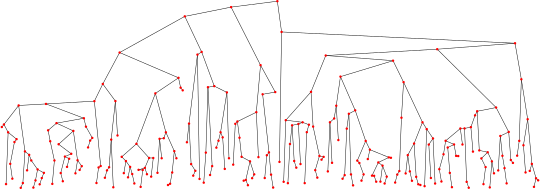
\includegraphics[scale=0.90909]{images/tree3-thick}}
%  \maketitle
%\end{titlepage}
%
%% blank page behind title page
%\ \thispagestyle{empty}\newpage
%
%\setcounter{page}{1}
%\chapter*{Acknowledgments}
\addcontentsline{toc}{chapter}{Acknowledgments}

I am grateful to Nima Hoda, who spent a summer tirelessly proofreading
many of the chapters in this book, and to the students in the Fall 2011
offering of COMP2402/2002, who put up with the first draft of this book
and spotted many typographic, grammatical, and factual errors in the
first draft.

%\ \thispagestyle{empty}\newpage
%\cpponly{\chapter*{Preface to the C++ Edition}
\addcontentsline{toc}{chapter}{Preface to the C++ Edition}

This book is intended to teach the design and analysis of basic data
structures and their implementation in an object-oriented language.
In this edition, the language happens to be C++.

This book is not intended to act as an introduction to the C++ programming
language.  Readers of this book need only be familiar with the basic
syntax of C++ and similar languages.  Those wishing to work with the
accompanying source code should have some experience programming in C++.

This book is also not intended as an introduction to the C++ Standard
Template Library or the generic programming paradigm that the STL
embodies.  This book describes implementations of several different data
structures, many of which are used in implementations of the STL. The
contents of this book may help an STL programmer understand how some of
the STL data structures are implemented and why these implementations
are efficient.

%\ \thispagestyle{empty}\newpage
%}

% Use 14pt between lines
\setlength{\baselineskip}{14pt}

\pagestyle{empty}

half title page
\newpage

series page
\newpage

title page
\newpage

\addtocontents{toc}{\protect\thispagestyle{empty}} % get rid of page number
\tableofcontents
\cleardoublepage

\fancyhead[RO,LE]{} % disable section numbers, for now
\pagestyle{fancy}
\chapter*{Acknowledgments}
\addcontentsline{toc}{chapter}{Acknowledgments}

I am grateful to Nima Hoda, who spent a summer tirelessly proofreading
many of the chapters in this book, and to the students in the Fall 2011
offering of COMP2402/2002, who put up with the first draft of this book
and spotted many typographic, grammatical, and factual errors in the
first draft.

\thispagestyle{empty}
\cleardoublepage

\fancyhead[CE]{\small Why This Book?} % chapter title, left center
\chapter*{Why This Book?}

There are plenty of books that teach introductory data structures.
Some of them are very good.  Most of them cost money, and the vast
majority of computer science undergraduate students will shell-out at
least some cash on a data structures book.

There are a few free data structures books available online.  Some are
very good, but most of them are getting old.  The majority of these
books became free when the author and/or publisher decided to stop
updating them.  Updating these books is usually not possible, for two
reasons:  (1)~The copyright belongs to the author or publisher, who
may not allow it.  (2)~The \emph{source code} for these books is often
not available.  That is, the Word, WordPerfect, FrameMaker, or \LaTeX\
source for the book is not available, and the version of the software
that handles this source may not even be available.

The goal of this project is to forever free undergraduate computer
science students from having to pay for an introductory data
structures book.  I have decided to implement this goal by treating
this book like an Open Source software project.  The \LaTeX\ source,
Java source, and build scripts for the book are available for download
on the book's website (\url{opendatastructures.org}) and also ---
more importantly --- on a reliable source code management site
(\url{https://github.com/patmorin/ods}).

This source code is released under a Creative Commons Attribution license,
meaning that anyone is free
\begin{itemize}
  \item to Share --- to copy, distribute and transmit the work; and
  \item to Remix --- to adapt the work.
\end{itemize}
This includes the right to make commercial use of the work.  The only
condition on these rights is
\begin{itemize}
  \item Attribution --- You must attribute the work by displaying a
  notice stating the derived work contains code and/or text from the
  Open Data Structures Project and/or linking to
  \url{opendatastructures.org}.
\end{itemize}

Anyone can contribute corrections/fixes using the \texttt{git} source-code
management system.  Anyone can fork from the current version of the
book and develop their own version (for example, in another programming
language).  They can then ask that their changes be merged back into
my version.  My hope is that, by doing things this way, this book will
continue to be a useful textbook long after my interest in the project
(or my pulse, whichever comes first) has waned.



\cleardoublepage

\fancyhead[CE]{\small\nouppercase{\leftmark}} % chapter title, left center
\fancyhead[RO,LE]{\small\textsection\thesection} % section number on the inside

\include{intro-lang}
\include{arrays-lang}
\include{linkedlists-lang}
\include{skiplists-lang}
\include{hashing-lang}
\include{binarytrees-lang}
\include{rbs-lang}
\include{scapegoat-lang}
\include{redblack-lang}
\include{heaps-lang}
\include{sorting-lang}
\include{graphs-lang}
\include{integers-lang}
\javaonly{
\include{btree-lang}
}

%% Turn off section numbers for remainder of document
\fancyhead[RO]{} % section number on the inside
\fancyhead[LE]{} % section number on the inside

\cleardoublepage
\addcontentsline{toc}{chapter}{Bibliography}
\bibliographystyle{abbrvurl}
\bibliography{ods,odsproc}

\cleardoublepage
\addcontentsline{toc}{chapter}{Index}
\printindex

\end{document}

